\section{Backend Komposition} \label{sec:backendComposition}

\subsection{Einführung in die Architektur} \label{sec:backendComposition:Introduction}
\begin{figure}
    \centering
    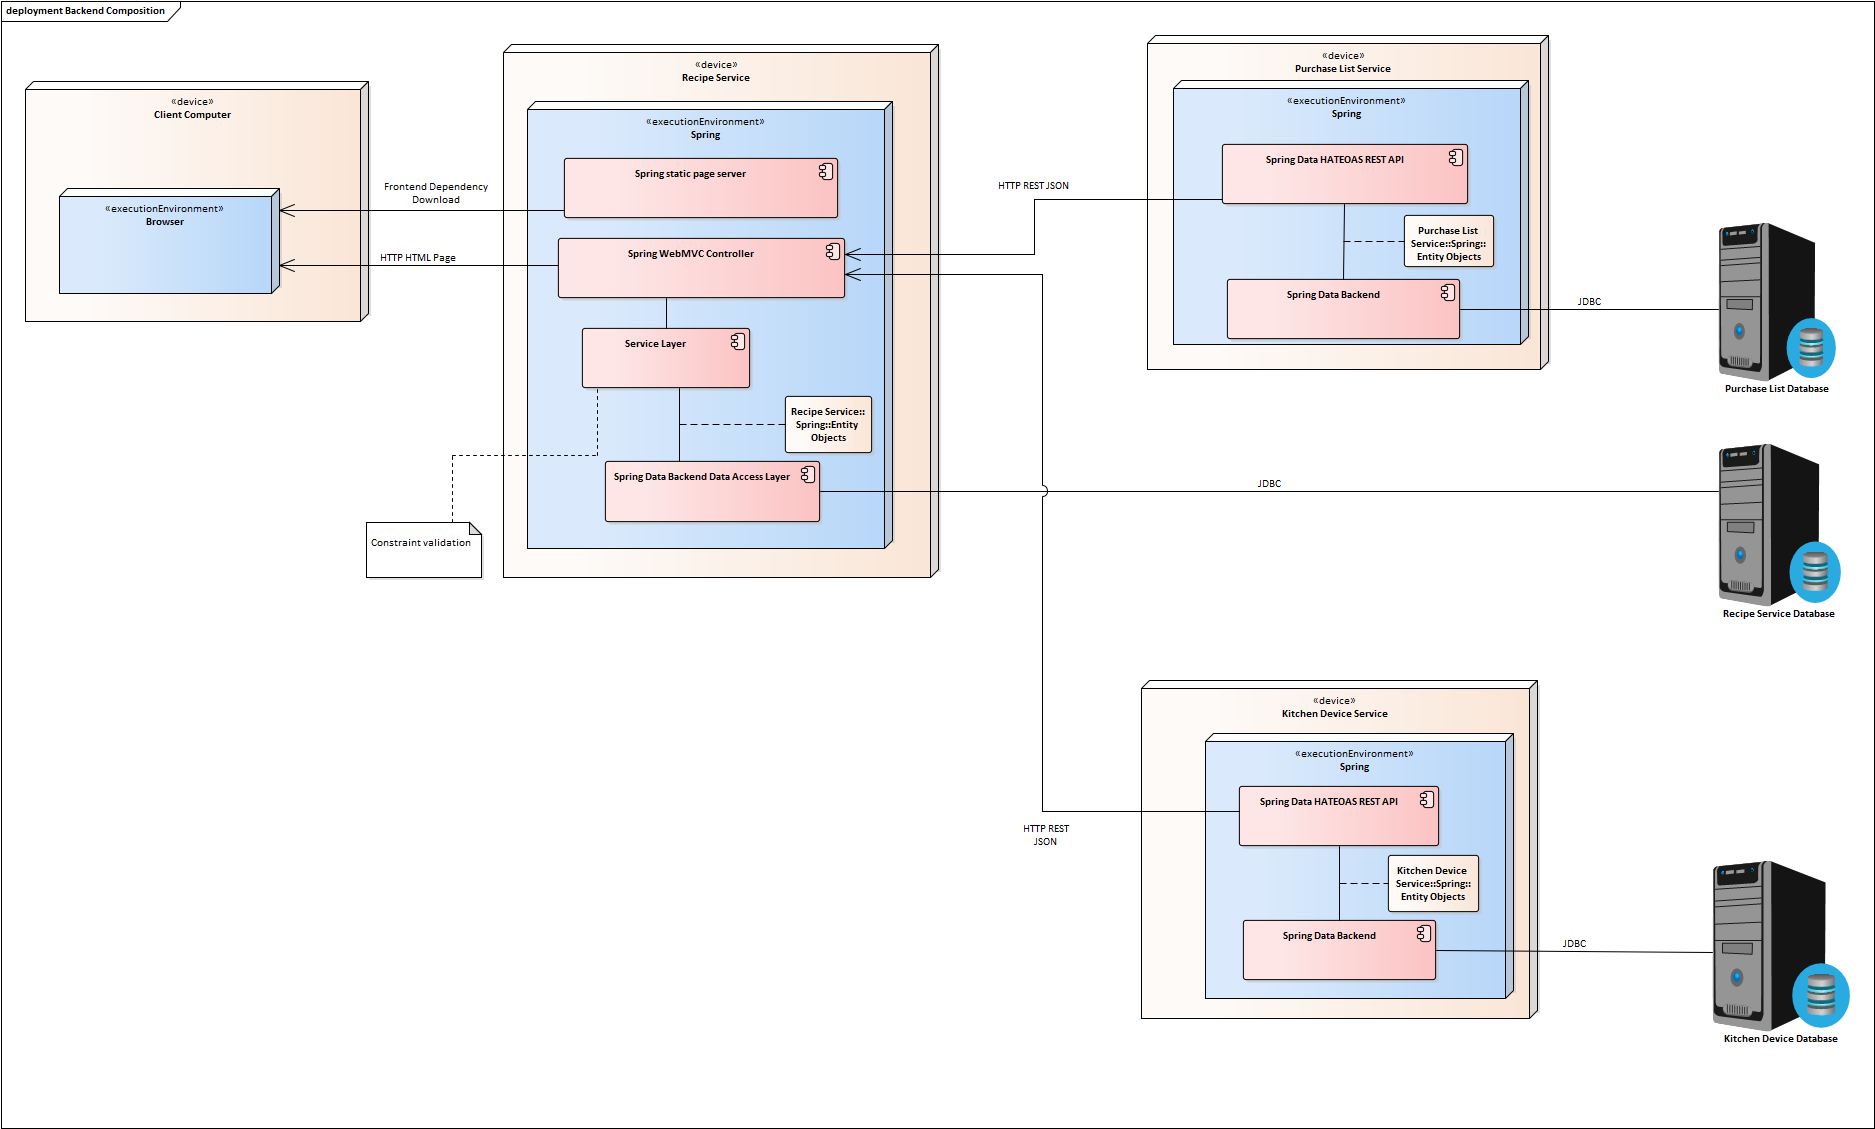
\includegraphics[width=\textwidth]{{sections/methology/assets/BackendComposition}}
    \caption{Backend Komposition}
    \label{fig:methology:backendComposition:Overview}
\end{figure}

Ein Kompositionsserver \marg{Architektur} führt die Daten der bestehenden Services in ein gemeinsames Frontend zusammen. Der Kompositionsserver kann Daten in verschiedenen Datenformaten erhalten und diese in ein HTML-Dokument rendern.

Die Alternative basiert auf dem Pattern \citetitle{RichardsonFragment} von \citeauthor{RichardsonFragment}.

Die Services \marg{Implikationen} müssen eine Schnittstelle zur Verfügung stellen über welche der Kompositionsserver auf die Daten des Services zugreifen kann. Diese Schnittstellen können unterschiedlichen Übertragungsprotokollen und Datenformaten besitzen.

Der Architekt erwartet folgende Vorteile durch die verwendete Alternative.
\begin{itemize}
    \pro Die Integration bedarf keine Änderungen an den Backendservices.
    \pro Die Integration kann mit verschiedenen Protokollen und Datenformaten umgehen.
\end{itemize}

Es wird erwartet, dass diese Risiken auftreten
\begin{itemize}
    \con Das Frontend ist in einem getrennten Projekt vom Backend Service.
    \con Die \ac{DTO} müssen auf dem Kompositionsserver und auf dem Backendservice gleichzeitig aktualisiert werden.
    \con Frontend Code und Backend Code werden auf zwei Projekte gespalten.
\end{itemize}

\subsection{Implementation der Architektur}

\begin{figure}
    \centering
    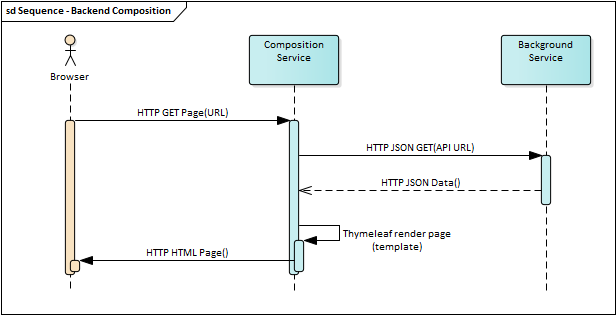
\includegraphics[width=\textwidth]{sections/methology/assets/SequenceBackendComposition}
    \caption{Interaktion bei Backend Komposition}
    \label{fig:sections:methology:backendComposition:Sequence}
\end{figure}

Abbildung \marg{Sequenz} \ref{fig:sections:methology:backendComposition:Sequence} zeigt das Sequenz-Diagramm der Implementierung von der Backend Komposition in der Beispielanwendung. Der Browser sendet einen HTTP GET Request an den Server. Der Server sendet einen \ac{REST}ful \ac{HTTP} Request für die Daten an den Backgroundservice. Nachdem der Backgroundservice die Daten geliefert hat, werden diese an Thymeleaf weitergegeben. Thymeleaf rendert ein Template mithilfe der empfangenen Daten und sendet das generierte Frontend an den Browser.

\begin{figure}
    \centering
\begin{lstlisting}
@GetMapping("/kitchenDevice/list")
public @NotNull Mono<ModelAndView> listKitchenDevice() {
    return kitchenDeviceService.get()
            .uri(KITCHEN_DEVICE_ROOT_PATH)
            .accept(MediaType.APPLICATION_JSON)
            .retrieve().bodyToMono(KitchenDeviceRoot.class)
            .map(kitchenDeviceRoot ->
                    new ModelAndView("kitchenDevice/list").addObject(PLURAL_MODEL_KEY, kitchenDeviceRoot)
            );
}
\end{lstlisting}
    \caption{BackendCompositionController.java}
    \label{fig:backendComposition:GETComposition}
\end{figure}

Der \marg{Implementation} Source-Code-Block \ref{fig:backendComposition:GETComposition} zeigt den Code für die Backend Komposition. Jede Frontend-Seite hat eine eigene Controller Methode im Kompositionsservice, die die Daten von den Backend Services lädt und das HTML-Dokument rendert. Diese muss für jede Seite auf dem Kompositionsserver spezifisch geschrieben werden.

\subsection{Resultate aus der Programmierung der Alternative}
Die Backend Komposition \marg{Chancen} stellte sich in der Implementation als sehr flexibel heraus. 

Die \marg{Risiken} Risiken liegen in der Duplizierung von Code zwischen dem Application und dem Kompositionsserver. Zum Beispiel müssen die \ac{DTO} auf beiden Servern auf gleichem Stand gehalten werden.

Der Architekt sieht ein Risiko bei der Aktualisierung des Übertragungsprotokolls, dass die Aktualisierung der \ac{DTO} des zweiten Services vergessen wird.

\subsection{Diskussion der Alternative}
Die Beispielimplementierung zeigt die Machbarkeit der Backend Composition auf. Ein Prototyp ist in dieser Arbeit erstellt worden. Anhand des Prototyps wurde dann der Kriterienvergleich ausgeführt.

Da jede Page eine eigene Controller Methode benötigt, ist es die Meinung des Architekten, dass die Backend Komposition Alternative eine Zentralisierung des Webservers darstellt. Das Frontend eines jeden Services wird herausgenommen und von dem Kompositionsserver ausgelieftert. Dies führt zu Risiken, die während der Implementierung der Alternative aufgetreten sind.

Die \marg{Erkenntnisse} Erwartungen des Architekten (siehe \ref{sec:backendComposition:Introduction}) haben sich in der Beispielapplikation gezeigt. Das Frontend liegt in einem getrennten Build-Projekt. Dadurch ist es vermehrt zu Versionskonflikten gekommen. Beispielsweise sind die \ac{DTO} nicht mehr aktuell gewesen auf dem Kompositionsserver. Auch der Umgekehrte Fall ist denkbar, wenn das Frontend verändert wird und der Applikationsserver nicht gleichzeitig aktualisiert wird.
\newpage